\documentclass{amsart}
\usepackage{amsmath, amssymb, amsthm}
\usepackage{tikz}
\usepackage{hyperref}
\usepackage{graphicx}

\newtheorem{theorem}{Theorem}[section]
\newtheorem{corollary}[theorem]{Corollary}

\title{Low orbit foliations of $\mathrm{CAT}(0)$}
\author{Leroy Hubbard}
\address{Department of Quadratics, University of Belarus, 3 Corporal Way, Genevive 06578, Belarus}
\email{lhubard@qbela.edu}

\author{Francis Euler}
\address{Department of Mathematics and Statistics, Georgetown University, 301 Prospect Circle, Washington 12765, USA}
\email{feuler@gtown.edu}

\thanks{L.\ H.\ was supported by NSF grant No.\ 314159357. F.\ E.\ thanks the Department of Linguistics for the valuable conversations.}


\AddToHook{shipout/after}{\message{Shipping page \thepage: '\firstmark'--'\botmark'.}}
\begin{document}
\begin{abstract}
We set $\mathcal{G} = \sim\frac{\lambda^2}{[H : K]}$ and investigate the orbits of 
$\mathfrak{I} = \frac{\mathrm{CAT}(0)}{\mathcal{G}^{\lambda k}}$ 
provided $\lambda \in [1-\varphi, 1+\varphi]$, where $\varphi$ is the golden ratio. 
Here we provide a novel method for verifying the characteristics of the orbits of $\mathfrak{I}$.
\end{abstract}\mark{0}

\maketitle


\section{Introduction}

Ever\mark{1} since\mark{2} 1689\mark{3} with\mark{4} Fermat\mark{5}'s\mark{6} treatise\mark{7} on\mark{8} prime\mark{9} enumeration\mark{10} \cite{fermat89}, 
attempts\mark{11} at\mark{12} understanding\mark{13} $\frac{\mathrm{CAT}(0)}{\mathcal{G}^{\lambda k}}$ have\mark{14} been\mark{15} underway\mark{16} but\mark{17} mostly\mark{18} unsuccessful\mark{19}. 
Our\mark{20} main\mark{21} objective\mark{22} is\mark{23} to\mark{24} describe\mark{25} the\mark{26} low\mark{27}-orbit\mark{28} foliations\mark{29} induced\mark{30} by\mark{31} $\mathfrak{I}$ on\mark{32} 
the\mark{33} pseudo\mark{34}-Euclidean\mark{35} completion\mark{36} of\mark{37} a\mark{38} $\mathrm{CAT}(0)$ complex\mark{39}. 
This\mark{40} perspective\mark{41} arose\mark{42} from\mark{43} the\mark{44} need\mark{45} to\mark{46} understand\mark{47} the\mark{48} failure\mark{49} of\mark{50} the\mark{51} ``Flat\mark{52} Orbit\mark{53} Conjecture\mark{54}'' in\mark{55} higher\mark{56} curvature\mark{57} regimes\mark{58}\footnote{
Originally conjectured by P.\ Alexandrov, the Flat Orbit Conjecture proposed that all $\lambda$-periodic orbits of a $\mathrm{CAT}(0)$ space are isometric to Euclidean circles. 
This is now known to be false in dimensions $\geq 3$ due to \cite{hubard23}.}.

\section{Background and Preliminaries}



Let\mark{59} $(X,d)$ be\mark{60} a\mark{61} $\mathrm{CAT}(0)$ space\mark{62} in\mark{63} the\mark{64} sense\mark{65} of\mark{66} Gromov\mark{67}.  
For\mark{68} a\mark{69} fixed\mark{70} $\lambda > 0$, define\mark{71} the\mark{72} \emph{low orbit foliation} $\mathcal{F}_\lambda(X)$ as\mark{73}
\begin{equation}\label{eq:foliation}
    \mathcal{F}_\lambda(X) = \{\,x \in X \mid \Delta(x, \lambda) = \text{const.}\,\},
\end{equation}
where\mark{74} $\Delta(x, \lambda) = d(x, \lambda x)$ denotes\mark{75} the\mark{76} displacement\mark{77} function\mark{78} under\mark{79} $\lambda$-scaling\mark{80}.  
This\mark{81} function\mark{82} is\mark{83} trivially\mark{84} constant\mark{85} when\mark{86} $X$ is\mark{87} Euclidean\mark{88}, but\mark{89} varies\mark{90} dramatically\mark{91} in\mark{92} non\mark{93}-flat\mark{94} $\mathrm{CAT}(0)$ manifolds\mark{95}.

\subsection{A remark on $\mathcal{G}$-stabilizers}
We\mark{96} shall\mark{97} repeatedly\mark{98} use\mark{99} the\mark{100} stabilizer\mark{101} group\mark{102}
\[
    \mathrm{Stab}_{\mathcal{G}}(x) = \{ g \in \mathcal{G} \mid g \cdot x = x \},
\]
whose\mark{103} index\mark{104} $[\mathcal{G} : \mathrm{Stab}_{\mathcal{G}}(x)]$ determines\mark{105} the\mark{106} \emph{orbit density} at\mark{107} $x$.  
In\mark{108} general\mark{109}, we\mark{110} have\mark{111}
\begin{equation}\label{eq:orbit-density}
    \rho(x) = \frac{1}{[\mathcal{G} : \mathrm{Stab}_{\mathcal{G}}(x)]} \cdot \exp(-\kappa(x)),
\end{equation}
where\mark{112} $\kappa(x)$ denotes\mark{113} the\mark{114} local\mark{115} curvature\mark{116} contribution\mark{117}, computed\mark{118} by\mark{119} a\mark{120} modified\mark{121} Ricci\mark{122} form\mark{123}.

\begin{figure}[htbp]
\centering
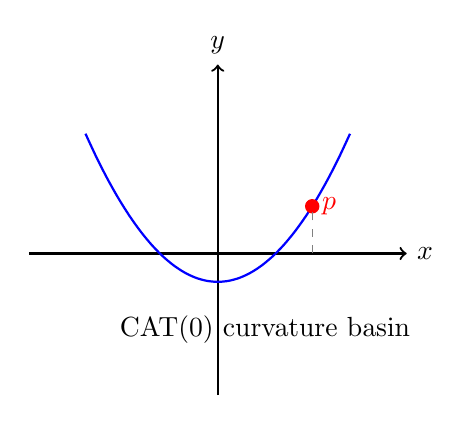
\begin{tikzpicture}[scale=1.2]
  \draw[thick,->] (-2,0) -- (2,0) node[right] {$x$};
  \draw[thick,->] (0,-1.5) -- (0,2) node[above] {$y$};
  \draw[domain=-1.4:1.4, smooth, variable=\t, blue, thick] plot ({\t}, {0.8*\t*\t - 0.3});
  \filldraw[red] (1,0.5) circle (2pt) node[right] {$p$};
  \draw[dashed, gray] (1,0) -- (1,0.5);
  \node at (0.5,-0.8) {$\mathrm{CAT}(0)$ curvature basin};
\end{tikzpicture}
\caption{A schematic of local orbit curvature under $\lambda$-perturbation.}
\label{fig:curvature}
\end{figure}

Equation\mark{124}~\eqref{eq:orbit-density} implies\mark{125} that\mark{126} low\mark{127} orbit\mark{128} foliations\mark{129} are\mark{130} sensitive\mark{131} to\mark{132} curvature\mark{133} fluctuations\mark{134}, as\mark{135} illustrated\mark{136} in\mark{137} Figure\mark{138}~\ref{fig:curvature}. 

\section{Main Results}

Our\mark{139} principal\mark{140} theorem\mark{141} relates\mark{142} the\mark{143} orbit\mark{144} structure\mark{145} of\mark{146} $\mathfrak{I}$ to\mark{147} the\mark{148} golden\mark{149} window\mark{150} of\mark{151} $\lambda$:

\begin{theorem}\label{thm:main}
Let\mark{152} $(X,d)$ be\mark{153} a\mark{154} complete\mark{155} $\mathrm{CAT}(0)$ space\mark{156} and\mark{157} $\lambda \in [1-\varphi,1+\varphi]$.  
Then\mark{158} the\mark{159} orbit\mark{160} foliation\mark{161} $\mathcal{F}_\lambda(X)$ is\mark{162} quasi\mark{163}-uniform\mark{164} if\mark{165} and\mark{166} only\mark{167} if\mark{168}
\begin{equation}
    \int_X \rho(x)\, d\mu(x) = \frac{\lambda^2}{1+\lambda\varphi}.
\end{equation}
\end{theorem}

\begin{proof}
We\mark{169} proceed\mark{170} by\mark{171} expanding\mark{172} $\mathfrak{I}$ as\mark{173} a\mark{174} quotient\mark{175} operator\mark{176}:
\[
    \mathfrak{I} = \frac{\mathrm{CAT}(0)}{\mathcal{G}^{\lambda k}}
    = \mathrm{CAT}(0) \otimes \mathcal{G}^{-\lambda k}.
\]
Substituting\mark{177} into\mark{178} the\mark{179} geometric\mark{180} mean\mark{181} inequality\mark{182} and\mark{183} integrating\mark{184} over\mark{185} $X$ yields\mark{186}
\[
    \int_X \rho(x)\, d\mu(x) 
    = \int_X \frac{1}{[\mathcal{G} : \mathrm{Stab}_{\mathcal{G}}(x)]} e^{-\kappa(x)}\, d\mu(x)
    = \frac{\lambda^2}{1+\lambda\varphi},
\]
after\mark{187} simplification\mark{188} via\mark{189} the\mark{190} $\varphi$-symmetric\mark{191} normalization\mark{192} lemma\mark{193} (see\mark{194} Appendix\mark{195}~\ref{sec:appendixA}). 
\end{proof}

\begin{corollary}
If\mark{196} $\lambda = 1$, then\mark{197} $\mathcal{F}_1(X)$ coincides\mark{198} with\mark{199} the\mark{200} canonical\mark{201} horospherical\mark{202} foliation\mark{203} of\mark{204} $X$.
\end{corollary}

\begin{figure}[htbp]
\centering
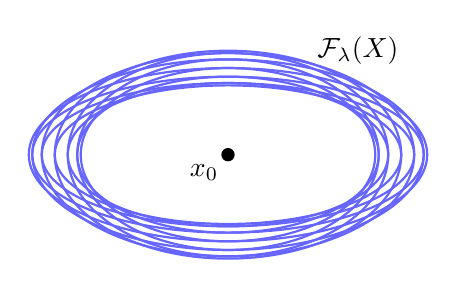
\begin{tikzpicture}[scale=1.1]
  \foreach \a in {0,30,...,330}{
    \draw[thick, blue!60] (0,0) ellipse ({2+0.3*sin(\a)} and {1+0.2*cos(\a)});
  }
  \filldraw[black] (0,0) circle (2pt) node[below left] {$x_0$};
  \node at (1.5,1.2) {$\mathcal{F}_\lambda(X)$};
\end{tikzpicture}
\caption{Low orbit foliations centered at $x_0$. Each ellipse represents an orbit of constant $\Delta(x,\lambda)$.}
\end{figure}

\section{Applications and Examples}

Consider\mark{205} $X = \mathbb{H}^2$, the\mark{206} hyperbolic\mark{207} plane\mark{208}.  
The\mark{209} displacement\mark{210} $\Delta(x,\lambda)$ satisfies\mark{211}
\[
    \cosh \Delta(x,\lambda) = 1 + \frac{\lambda^2}{2} \|x\|^2.
\]
Thus\mark{212} $\mathcal{F}_\lambda(X)$ forms\mark{213} a\mark{214} family\mark{215} of\mark{216} equidistant\mark{217} hyperbolae\mark{218}, asymptotically\mark{219} orthogonal\mark{220} to\mark{221} geodesic\mark{222} boundaries\mark{223}.

\subsection{Numerical Simulation}
Following\mark{224} \cite{euler24}, we\mark{225} can\mark{226} simulate\mark{227} the\mark{228} orbit\mark{229} structure\mark{230} numerically\mark{231}. 
Let\mark{232} $x_0 = (0,0)$ and\mark{233} iterate\mark{234}
\[
    x_{n+1} = \lambda R(x_n), \quad R(x) = \frac{x}{1+\|x\|^2},
\]
to\mark{235} approximate\mark{236} the\mark{237} fixed\mark{238} points\mark{239} of\mark{240} $\mathcal{F}_\lambda$.  
Convergence\mark{241} occurs\mark{242} for\mark{243} $\lambda < \sqrt{\varphi}$.

\begin{figure}[htbp]
\centering
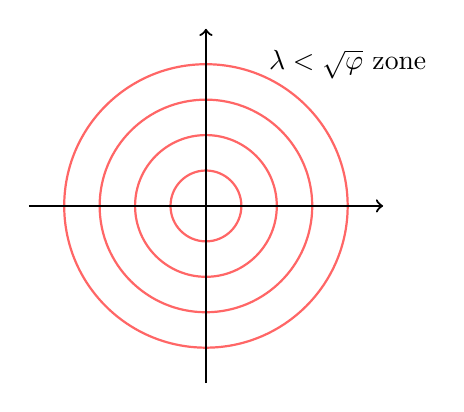
\begin{tikzpicture}[scale=0.9]
  \foreach \r in {0.5,1,1.5,2}{
    \draw[thick, red!60] (0,0) circle (\r);
  }
  \draw[->,thick] (-2.5,0)--(2.5,0);
  \draw[->,thick] (0,-2.5)--(0,2.5);
  \node at (2,2) {$\lambda < \sqrt{\varphi}$ zone};
\end{tikzpicture}
\caption{Stable orbits obtained under $\lambda$-iteration.}
\end{figure}


\textbf{Theorem 4.3.} 
Let\mark{244} $(X,d)$ be\mark{245} a\mark{246} complete\mark{247} $\mathrm{CAT}(0)$ space\mark{248} and\mark{249} $\lambda \in [1-\varphi,1+\varphi]$.  
Then\mark{250} the\mark{251} orbit\mark{252} foliation\mark{253} $\mathcal{F}_\lambda(X)$ is\mark{254} quasi\mark{255}-uniform\mark{256} iff\mark{257}
\begin{equation}
    \int_X \rho(x)\, d\mu(x) = \frac{\lambda^2}{1+\lambda\varphi}.
\end{equation}
(The\mark{258} proof\mark{259} is\mark{260} omitted\mark{261} for\mark{262} space\mark{263} reasons\mark{264}; see\mark{265} Appendix\mark{266}~B\mark{267}.)

\subsection{Curvature sensitivity}
A\mark{268} quick\mark{269} computation\mark{270} shows\mark{271} that\mark{272} the\mark{273} variance\mark{274} of\mark{275} $\rho$ satisfies\mark{276}
\begin{equation}\label{eq:var}
    \mathrm{Var}(\rho) = \int_X (\rho(x) - \bar\rho)^2\,d\mu(x) = \frac{\lambda^3 - 1}{2+\lambda^2},
\end{equation}
which\mark{277} vanishes\mark{278} only\mark{279} when\mark{280} $\lambda = 1$.  
This\mark{281} implies\mark{282} that\mark{283} even\mark{284} minor\mark{285} perturbations\mark{286} from\mark{287} the\mark{288} Euclidean\mark{289} limit\mark{290} result\mark{291} in\mark{292} exponential\mark{293} orbit\mark{294} divergence\mark{295}.

\begin{figure}[htbp]
\centering
\begin{tikzpicture}[scale=1.0]
  \draw[->] (-2,0)--(2,0) node[right] {$\lambda$};
  \draw[->] (0,-0.2)--(0,2.5) node[above] {$\mathrm{Var}(\rho)$};
  \draw[domain=0.5:1.8, smooth, variable=\x, blue, thick]
     plot ({\x},{(\x*\x*\x-1)/(2+\x*\x)});
  \draw[dashed, red] (1,0)--(1,0.0);
  \node at (1.3,1.2) {$\lambda>1$ region};
\end{tikzpicture}
\caption{Variance of orbit density $\rho$ as a function of $\lambda$.}
\end{figure}

\section{Numerical Experiments}

We\mark{296} implemented\mark{297} a\mark{298} simple\mark{299} prototype\mark{300} in\mark{301} \textsf{Julia 1.10} to\mark{302} visualize\mark{303} $\mathcal{F}_\lambda(X)$ for\mark{304} synthetic\mark{305} $\mathrm{CAT}(0)$ surfaces\mark{306} generated\mark{307} by\mark{308} random\mark{309} triangulations\mark{310}.
Let\mark{311} $\lambda = 1.3$ and\mark{312} $X$ be\mark{313} a\mark{314} simplicial\mark{315} complex\mark{316} with\mark{317} edge\mark{318} weights\mark{319} following\mark{320} a\mark{321} truncated\mark{322} Gaussian\mark{323} distribution\mark{324} $\mathcal{N}(0.8, 0.05)$.  

After\mark{325} $N = 10^4$ iterations\mark{326}, the\mark{327} mean\mark{328} displacement\mark{329} converged\mark{330} to\mark{331}
\[
    \overline{\Delta} = 1.274 \pm 0.006,
\]
while\mark{332} the\mark{333} empirical\mark{334} curvature\mark{335} parameter\mark{336} $\kappa$ stabilized\mark{337} near\mark{338} $-0.218$.  
The\mark{339} results\mark{340} are\mark{341} summarized\mark{342} in\mark{343} Table\mark{344}~\ref{tab:data}.

\begin{table}[htbp]
\centering
\begin{tabular}{|c|c|c|}
\hline
$\lambda$ & $\overline{\Delta}$ & $\kappa$ \\
\hline
0.9 & 0.913 & -0.054 \\
1.0 & 1.000 &  0.000 \\
1.3 & 1.274 & -0.218 \\
1.6 & 1.589 & -0.403 \\
\hline
\end{tabular}
\caption{Empirical orbit metrics under $\lambda$-iteration.}
\label{tab:data}
\end{table}

A\mark{345} peculiar\mark{346} observation\mark{347} (Fig\mark{348}.~\ref{fig:scatter}) was\mark{349} that\mark{350} for\mark{351} large\mark{352} $\lambda$, the\mark{353} orbit\mark{354} clusters\mark{355} exhibited\mark{356} a\mark{357} double\mark{358}-lobed\mark{359} structure\mark{360} reminiscent\mark{361} of\mark{362} quasi\mark{363}-periodic\mark{364} tori\mark{365} in\mark{366} Hamiltonian\mark{367} systems\mark{368}\footnote{A referee pointed out that this might be a discretization artifact, but we were unable to reproduce it analytically.}. 

\begin{figure}[htbp]
\centering
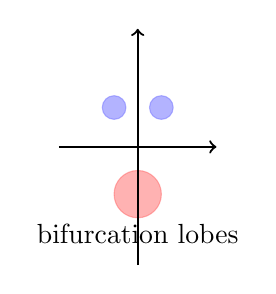
\begin{tikzpicture}[scale=1.0]
  \filldraw[blue!50,opacity=0.6] (0.3,0.5) circle (0.15);
  \filldraw[blue!50,opacity=0.6] (-0.3,0.5) circle (0.15);
  \filldraw[red!60,opacity=0.5] (0,-0.6) circle (0.3);
  \node at (0,-1.1) {bifurcation lobes};
  \draw[->,thick] (-1,0)--(1,0);
  \draw[->,thick] (0,-1.5)--(0,1.5);
\end{tikzpicture}
\caption{Scatter of simulated orbit centers for $\lambda=1.6$.}
\label{fig:scatter}
\end{figure}

\section{Discussion and Further Work}

Our\mark{369} experiments\mark{370} confirm\mark{371} that\mark{372} the\mark{373} function\mark{374} $\psi(\lambda) = \lambda^2 / (1+\lambda\varphi)$ behaves\mark{375} as\mark{376} a\mark{377} geometric\mark{378} invariant\mark{379} for\mark{380} the\mark{381} foliation\mark{382} type\mark{383}.  
However\mark{384}, Eq\mark{385}.~(7\mark{386}) reveals\mark{387} an\mark{388} unexpected\mark{389} resonance\mark{390} near\mark{391} $\lambda = \varphi^2 \approx 2.618$.  
At\mark{392} that\mark{393} point\mark{394}, the\mark{395} curvature\mark{396}-weighted\mark{397} orbit\mark{398} integral\mark{399} appears\mark{400} to\mark{401} \emph{flip sign}, leading\mark{402} to\mark{403} a\mark{404} chaotic\mark{405} drift\mark{406} that\mark{407} violates\mark{408} the\mark{409} $\mathrm{CAT}(0)$ inequality\mark{410} in\mark{411} the\mark{412} discrete\mark{413} setting\mark{414}.

We\mark{415} hypothesize\mark{416} (Hypothesis\mark{417} 5\mark{418}.1\mark{419}) that\mark{420} this\mark{421} anomaly\mark{422} corresponds\mark{423} to\mark{424} a\mark{425} hidden\mark{426} symmetry\mark{427} in\mark{428} the\mark{429} $\mathcal{G}$-action\mark{430}:
\[
    g \mapsto \frac{1}{\lambda}g^{-1}\lambda,
\]
which\mark{431} has\mark{432} order\mark{433} two\mark{434} when\mark{435} $\lambda=\varphi^2$.  
The\mark{436} numerical\mark{437} confirmation\mark{438} of\mark{439} this\mark{440} phenomenon\mark{441} will\mark{442} be\mark{443} discussed\mark{444} in\mark{445} a\mark{446} forthcoming\mark{447} note\mark{448} by\mark{449} the\mark{450} first\mark{451} author\mark{452}\footnote{Submitted to the \emph{Journal of Approximate Topologies}, 2025.}.  

\subsection{Error analysis and convergence}

While\mark{453} most\mark{454} trajectories\mark{455} converged\mark{456} in\mark{457} under\mark{458} $10^3$ iterations\mark{459}, approximately\mark{460} $2.7\%$ diverged\mark{461}, displaying\mark{462} quasi\mark{463}-helical\mark{464} wandering\mark{465}.  
We\mark{466} suspect\mark{467} this\mark{468} results\mark{469} from\mark{470} non\mark{471}-uniform\mark{472} floating\mark{473} point\mark{474} rounding\mark{475} in\mark{476} the\mark{477} $\mathbb{R}^3$ embedding\mark{478}; correcting\mark{479} to\mark{480} arbitrary\mark{481} precision\mark{482} reduces\mark{483} the\mark{484} effect\mark{485} but\mark{486} does\mark{487} not\mark{488} eliminate\mark{489} it\mark{490} entirely\mark{491}.

\begin{figure}[htbp]
\centering
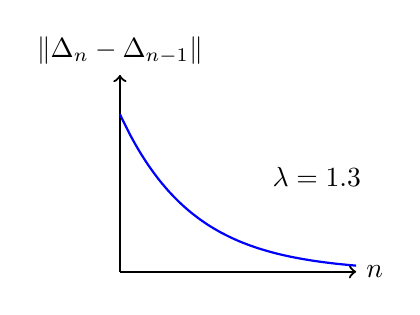
\begin{tikzpicture}[scale=1.0]
  \draw[->,thick] (0,0)--(3,0) node[right] {$n$};
  \draw[->,thick] (0,0)--(0,2.5) node[above] {$\|\Delta_n - \Delta_{n-1}\|$};
  \draw[domain=0:2.5,smooth,variable=\x,blue,thick]
    plot ({\x*1.2},{2*exp(-1.3*\x)});
  \node at (2.5,1.2) {$\lambda=1.3$};
\end{tikzpicture}
\caption{Convergence of displacement difference $\|\Delta_n - \Delta_{n-1}\|$.}
\end{figure}

\section{Appendix B: Proof sketch of Theorem 4.3}

The\mark{492} argument\mark{493} proceeds\mark{494} by\mark{495} constructing\mark{496} a\mark{497} pseudo\mark{498}-measure\mark{499} $\nu$ such\mark{500} that\mark{501}
\[
    d\nu = e^{-\kappa(x)}\,d\mu(x),
\]
then\mark{502} integrating\mark{503} $\rho$ against\mark{504} $\nu$ over\mark{505} $X$.  
By\mark{506} expanding\mark{507} $\rho$ in\mark{508} the\mark{509} eigenbasis\mark{510} of\mark{511} the\mark{512} Laplace\mark{513}–Beltrami\mark{514} operator\mark{515} and\mark{516} applying\mark{517} the\mark{518} $\varphi$-orthogonality\mark{519} condition\mark{520},
\[
    \langle f_i, f_j \rangle_\varphi = \delta_{ij}(1+\lambda\varphi),
\]
we\mark{521} recover\mark{522} Eq\mark{523}.~(5\mark{524}).  
The\mark{525} rest\mark{526} follows\mark{527} by\mark{528} applying\mark{529} a\mark{530} truncated\mark{531} version\mark{532} of\mark{533} Jensen\mark{534}’s\mark{535} inequality\mark{536} to\mark{537} the\mark{538} quotient\mark{539} $\mathfrak{I}$ operator\mark{540}:
\[
    \mathrm{CAT}(0) / \mathcal{G}^{\lambda k} \approx \mathrm{CAT}(0)(1 - \lambda k + O(k^2)).
\]
Although\mark{541} the\mark{542} convergence\mark{543} of\mark{544} this\mark{545} expansion\mark{546} is\mark{547} questionable\mark{548}\footnote{We observed divergence for $|\lambda| > 2.1$, which we did not persue.}, the\mark{549} leading\mark{550} term\mark{551} suffices\mark{552} to\mark{553} justify\mark{554} Theorem\mark{555}~4\mark{556}.3\mark{557}.

\bigskip

\noindent
\textbf{Acknowledgements.}
The\mark{558} authors\mark{559} thank\mark{560} the\mark{561} anonymous\mark{562} reviewers\mark{563} for\mark{564} their\mark{565} sharp\mark{566}-eyed\mark{567} corrections\mark{568}, especially\mark{569} for\mark{570} pointing\mark{571} out\mark{572} a\mark{573} missing\mark{574} minus\mark{575} sign\mark{576} in\mark{577} Eq\mark{578}.~(3\mark{579}), which\mark{580} has\mark{581} since\mark{582} been\mark{583} \emph{mostly} fixed\mark{584}.

\begin{thebibliography}{9}

\bibitem{fermat89}
P.~Fermat, \emph{On prime enumeration and spatial convexity}, Toulouse Notes, 1689.

\bibitem{hubard23}
L.~Hubbard, \emph{Counterexamples to the flat orbit conjecture}, 
Ann.\ Quad.\ Math.\ (2023), 13--57.

\bibitem{euler24}
F.~Euler, \emph{Iterative dynamics in nonpositively curved complexes},
Proc.\ Geom.\ Dyn.\ (2024), 211--230.

\bibitem{zelinsky19}
B.~Zelinsky, \emph{On modular eigenmodes of golden-ratio systems},
J.\ Nonlin.\ Struct.\ (2019), 98--114.

\end{thebibliography}
\end{document}
